\documentclass[12pt]{article}

\usepackage[francais]{babel}
\usepackage[utf8]{inputenc}
\usepackage[T1]{fontenc}
\usepackage[left=2cm,right=2cm,top=2cm,bottom=2cm]{geometry}
\usepackage{amsmath}
\usepackage{graphicx}
\usepackage{pdfpages}

\begin{document}
\begin{titlepage}

\newcommand{\HRule}{\rule{\linewidth}{0.5mm}} % Défini une nouvelle commande pour faire une ligne horizontale. Changer l'épaisseur se fait ici.

\center % Centre tout dans la page.

%----------------------------------------------------------------------------------------
%   HEADING SECTIONS
%----------------------------------------------------------------------------------------

\textsc{\LARGE Université de Rouen}\\[1.5cm]
\textsc{\Large Amicale GIL}\\[0.5cm]
\textsc{\large Master 1}\\[0.5cm]

%----------------------------------------------------------------------------------------
%   TITLE SECTION
%----------------------------------------------------------------------------------------

\HRule \\[0.4cm]
{ \huge \bfseries Projet architecture logiciel}\\[0.2cm] % Titre du document.
\HRule \\[1.5cm]
  

%----------------------------------------------------------------------------------------
%   DATE SECTION
%----------------------------------------------------------------------------------------

  {\large Date : \today}\\
  
  
%----------------------------------------------------------------------------------------
%   AUTHOR SECTION
%----------------------------------------------------------------------------------------
  \vfill % Fill the rest of the page with whitespace
  
  \begin{minipage}{0.6\textwidth} \large
  	\begin{flushleft}
  		\emph{Effectué par:} \\
  		\textsc{FLEURY} Yoann \& \textsc{CROCHEMORE} Valentin
  	\end{flushleft}
  \end{minipage}\\[2cm]


  
\end{titlepage}

\newpage
\tableofcontents
\newpage

\section{Architecture de l'application}
\label{sec:arch_app}

	L'application est découpée en plusieurs parties : 
	\begin{itemize}
		\item La partie test, avec les différents tests demandés.
		\item La partie façade, qui se charge de faire la liaison entre la partie test et la partie gestionnaire de paramètre.
		\item La partie gestionnaire de paramètre qui comporte deux sous-parties :
		\begin{itemize}
			\item La partie d'écriture/lecture des paramètres
			\item La partie gestion des clés
		\end{itemize}
	\end{itemize}
	\subsection{La partie test}
	
	En ce qui concerne la partie test, il n'y a rien de particulier à dire, chaque test a sa propre classe.
	
	\subsection{La partie façade}

	Comme son nom l'indique, cette partie utilise le patron \textbf{façade} afin de "cacher" le fonctionnement des autres parties, de faciliter l'accès au sous système et permet aussi de fournir seulement les classes nécessaires à l'exécution du client.
	
	\paragraph{}
	Le client ne sachant pas comment fonctionne le sous système, il est tout à fait possible de modifier son fonctionnement (sans changer le résultat) sans paralyser le client, par exemple si l'on veut optimiser le sous système ou changer de format d'enregistrement des paramètres. Les méthodes appelées par le client sont des redirections vers les méthodes du sous système désirées. Cela donne une certaine modularité au sous système.
	
	\paragraph{}
	Le patron \textbf{façade} permet de faciliter l'accès au sous système, celui-ci n'est pas compliqué d'accès, cependant en prévention d'une évolution (en taille mais aussi en complexité). Nous avons jugé que le coup de cette implémentation été minime par rapport aux gains quelle pourrait apporter.
	
	\paragraph{}
	Le patron a aussi permis de donner au client l'accès à la seule classe qui lui est nécessaire pour son bon fonctionnement. Nous avons donc mis en place deux façades, chaque façade est formée par un couple interface/classe, un couple permettant seulement la "lecture seule" des réglages et couple permettant la lecture et l'écriture. Il serais tout à fait possible de rajouter un troisième couple permettant seulement l'écriture. Cela cloisonne l'accès aux classes et évite de fournir au client plus que nécessaire à son bon fonctionnement. 
	
	\newpage
	\subsection{La partie gestionnaire de paramètre}
	
	Pour cette partie il fallait avoir une modularité assez importante afin que l'application puisse évoluer le plus facilement possible, c'est-à-dire limiter le nombre de modification de l'existant au stricte minimum.
	
	\subsubsection{La partie lecture/écriture}
	
		Pour cette partie nous avons mis en place un patron proche du patron \textbf{pont}, dans son principe, c'est-à-dire le découplage de la partie lecture/écriture. Cela permet aux deux parties d'évoluer de manière indépendantes, et d'ajouter un lecteur sans forcément ajouter d'écrivain et inversement. Cela permet aussi de faciliter le changement du type de sauvegarde des réglage (XML, XHTML ...). De plus nous avons mis en place une interface permettant aux classes plus haut niveau de manipuler des \verb+Reader+ et \verb+Writer+ sans savoir si il s'agit de \verb+ReaderJSON+ ou \verb+ReaderXML+ par exemple. Il est donc simple de changer de format de sauvegarde.
		
	\subsubsection{La partie gestion des clés}
	
		Pour cette partie nous avons utilisé la patron \textbf{composite}. En effet les clés de paramètre étant découpées en deux (des clés de groupe et des clés de valeur), une clé de groupe peut contenir une autre clé de groupe ou une clé de valeur, cela correspond parfaitement au patron \textbf{composite}. Les clés de valeur sont donc considérées comme des feuilles et les clés de groupe comme des component. Ce patron permet au système de traiter ces deux types de clé de la même manière. Ainsi chaque clés connait la façon de s'afficher en interne ce qui simplifie l'affichage des réglages.
\section{Fonctions implémentées}
\label{sec:fonctions_impl}

\begin{itemize}
	\item Demander le chargement de l’ensemble des réglages à partir d’un fichier.
	\item Demander la sauvegarde de l’ensemble des réglages vers un fichier.
	\item Obtenir une valeur à partir de sa clé de réglage.
	\item Ajouter ou modifier une valeur à partir de sa clé de réglage et d’une nouvelle valeur.
	\item Supprimer une valeur à partir de sa clé de réglage.
	\item Obtenir une référence à un groupe à partir sa clé de groupe.
	\item Supprimer un groupe à partir sa clé de groupe.
	\item Accéder à un groupe ou une valeur de manière relative, c'est à dire à partir d’un autre groupe.
\end{itemize}

\section{Fonctions non implémentées}
\label{sec:fonctions_non_impl}
Toutes les fonctionnalités ont été implémentées.

\section{Schéma UML}
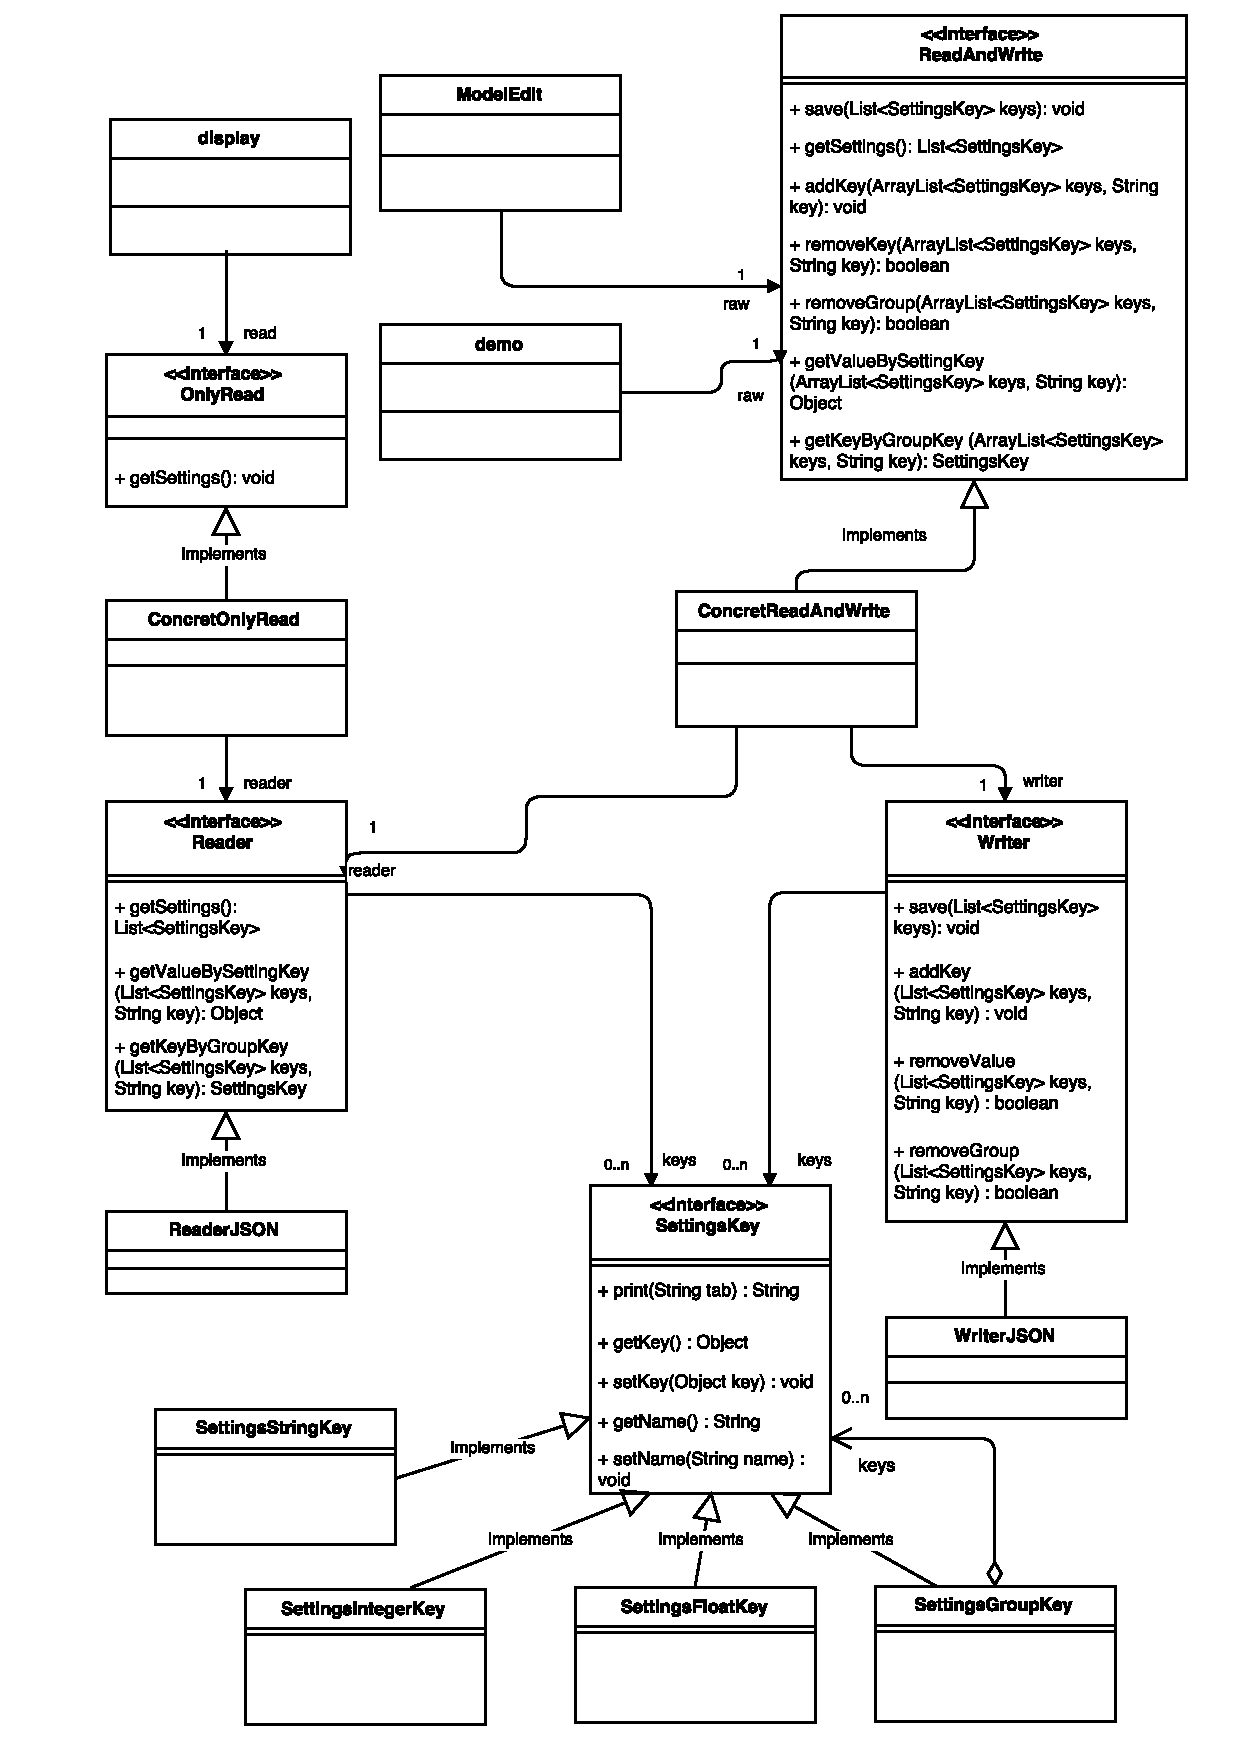
\includepdf[pages={1}]{DiagrammeUML.pdf}
\end{document}
